\excercise{Klassendiagramm des \simulator{}s}

\Todo{Update the class diagram}
\Todo{Rework task abd maybe move to later}
% Alle Methoden eines Objekts finden
% Ursprungsklasse für eine Methode finden
% Learning goal: Eine API verstehen

\Todo{Neue Aufgabe: Doku lesen}
% Doku für eine Methode (die move methode) finden (oder direkt angeben) und dann verschiedene Beispiele auf dem Blatt (normal ohne hinderniss laufen, dann gegen hinderniss laufen) entscheiden lassen ob es funktioniert.
% Playground bereitstellen in denen sie ihre vermutung ausprobieren können
% Learning goal: Javadoc finden, lesen und logisch anwenden (und überprüfen)

Hier (im Bild auf der nächsten Seite) ist das Klassendiagramm von unserem Simulator:

    Die Pfeile zeigen dabei an, dass die Klasse von der der Pfeil ausgeht alle Attribute und Operationen der Klasse auf die der Pfeil zeigt auch hat.
    Das ist zwar sehr vereinfacht ausgedrückt, da hier nicht nur Klassen sondern auch Interfaces im Klassendiagramm dargestellt sind und auch die unterschiedlichen Pfeile etwas andere Bedeutungen haben, aber es genügt um das Klassendiagramm grob zu verstehen.
    Eine \texttt{GreedyEntity} hat also auch die Operation \texttt{move()} die in \texttt{MoveableEntity}.
    Das gilt übrigens auch für \texttt{Neo} (über \texttt{Human}, \texttt{GreedyEntity} zu \texttt{MoveableEntity}).


        \subexcercise Liste alle Operationen von der Klasse \texttt{Coin} auf.
        \subexcercise Entscheide für Operationen die direkt in der Klasse \texttt{MoveableEntity} definiert sind ob es sich um eine Query oder ein Kommando handelt.
        \subexcercise Finde die Klasse \texttt{Neo} in dem Projekt.
            In welchem Ordner ist die Klasse?
            In welchem Paket ist die Klasse?
        \subexcercise Finde die Klasse die zu der Aufgabe \fbox{Task0 a)} den du vorher gestartet hast gehört.
            Hinweis: Schau dir die \texttt{Main} Klasse gut an.
            Wenn du eine \texttt{solve()} Operation mit dem Kommentar \texttt{// do AB1 task 5 \& 6 here} siehst bist du richtig.


    \makebox[\linewidth][c]{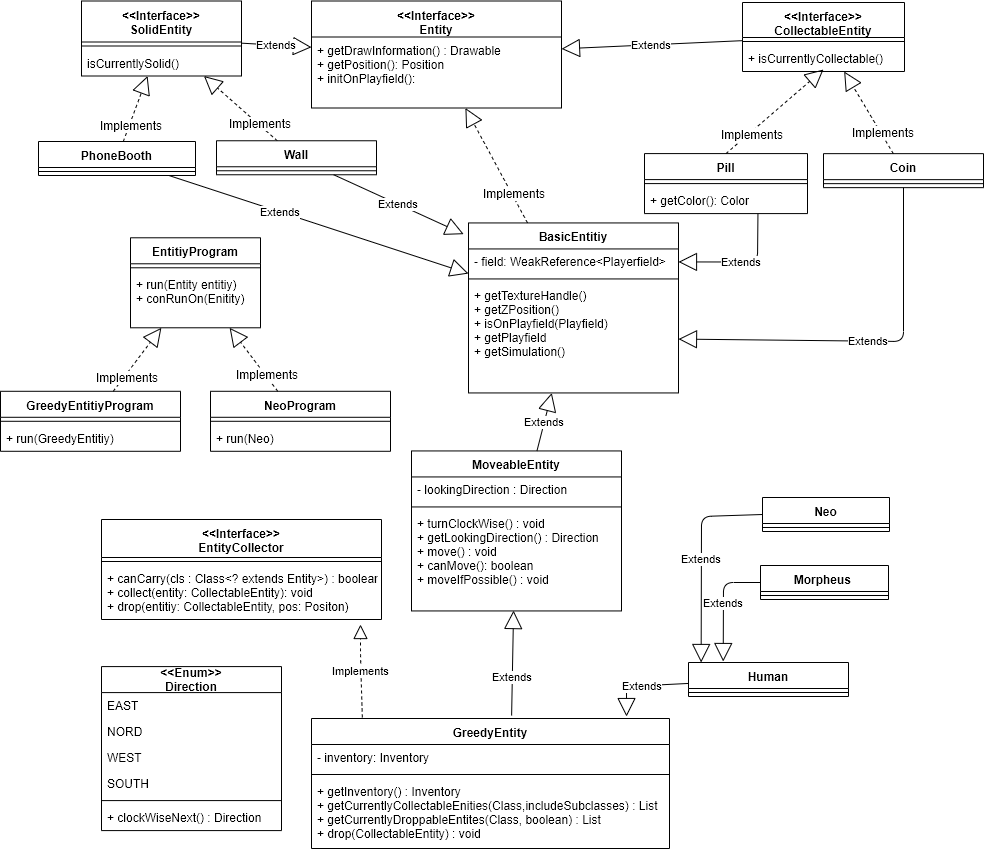
\includegraphics[width=1.2\textwidth]{figures/icge-class-diagramm.png}}
